\documentclass[a4paper, oneside, 11pt, pointlessnumbers, headsepline, bibtotoc]{scrbook}

% Get the necessary packages for the document.
% Set to english language and utf8.
\usepackage[english]{babel}
\usepackage[utf8]{inputenc}

% Some packages for symbols we need within the tutorial.
\usepackage{dingbat}
\usepackage{marvosym}

% For the sourcecode.
\usepackage{listings}

% Enable Jan's highlighting
% Usage:
% %% preamble
% \usepackage{listings} %% correct name?
\usepackage{lstide}
% \lstset{tabsize=2,captionpos=b,style=default,}
%
%
% %% main
%     \begin{lstlisting}[style=eclipse-java,gobble=6,caption={Simple micro-benchmark in Java}]
%       for (int i = 0; i < 1000; i++) {
%         tin = currentTime();
%         benchmarkedOperation // testtext
%         tout = currentTime();
%       }
%     \end{lstlisting}

% For the links etc.
\usepackage{hyperref} % avh: removed [pdfborder={0 0 0}]

% For the pdf-graphics.
\usepackage{graphicx}

% The steamroller tactics to fix figures and so on.
\usepackage{float}

% This is for tables which are to long to be shown on one page.
\usepackage{longtable}

% This package is for the directory tree structures
\usepackage{dirtree}
\renewcommand*\DTstylecomment{\footnotesize\normalfont\itshape\rmfamily}
\renewcommand*\DTstyle{\footnotesize\sffamily}

% We need this package for some color within the document.
\usepackage{color}

\usepackage[sort,compress,numbers]{natbib} %round,authoryear

% compactitem, compactenum, ...
\usepackage{paralist}


% This is the package for the margin-nodes.
\usepackage[color=white, bordercolor=white]{todonotes}

\usepackage{amsfonts}
\usepackage{setspace}
\usepackage{ae,aecompl}

\usepackage[automark]{scrpage2}

\usepackage[margin=0.5cm,indention=0em,font={small},labelfont={sf,small},format=hang]{caption}

\usepackage[hang,sf]{subfigure}
\subfigcapmargin=1em

%\usepackage{scrhack}

% Get the new commands we defined for this document.
\newcommand{\Kieker}{\textit{Kieker}}
\newcommand{\home}{$\sim$}

\pagestyle{scrheadings}
\clearscrheadfoot

\ifoot[\hrule\sffamily Kieker \version{} User Guide]{\hrule\sffamily Kieker \version{} User Guide}
\ofoot[\hrule\sffamily\pagemark]{\hrule\sffamily\pagemark} 

% Set the title and everything.
\titlehead{
	\begin{center}
		\includegraphics[height=25mm]{./images/kieker-logo}\\
\href{http://kieker.sourceforge.net}{\sffamily\Large http://kieker.sourceforge.net}
	\end{center}
}

\title{%
\Huge\Kieker{} \version{} User Guide%
}

\author{\sffamily Nils Ehmke, Andr\'e van Hoorn%
\footnote{\sffamily Corresponding author; e-mail: \texttt{avh@informatik.uni-kiel.de}}%
, and Reiner Jung} % , and contributors
%\date{\sffamily\today}
\date{\sffamily May 19, 2011}
\publishers{\normalsize\sffamily
%\flushleft
\includegraphics[height=2.5cm]{./images/caulogo}\\[0.5ex]
Software Engineering Group, \url{http://se.informatik.uni-kiel.de}\\ %
Dept.\ Computer Science, Christian Albrechts University of Kiel, Germany
}

\hypersetup
{%
pdftitle = {\Kieker{} \version{} User Guide},
pdfauthor = {Nils Ehmke, Andr\'e van Hoorn, and Reiner Jung}
% colorlinks = {true}
}

% Here we go.
\begin{document}
  % We want a table of contents separated from the rest of the text.
  \maketitle
  \setcounter{tocdepth}{1} % not deeper than section level
  {\sffamily\tableofcontents}

  % Insert the other parts of the document.
  %%%%%%%%%%%%%%%%%%%%%%%%%%%%%%%%%%%%%%%%%
% Introduction
%
% $Date$
% $Revision$
% $Author$


\chapter{Introduction}\label{chap:introduction}

Modern software applications are often complex and have to fulfill a large set of functional and non-functional requirements. The internal behavior of such large systems cannot easily be determined on the basis of the source code. Furthermore, existing applications often lack sufficient documentation which makes it cumbersome to extend and change them for future needs. A solution to these problems can be dynamic analysis based on application-level monitoring, which allows to log the behavior of the application and to discover, for example, application-internal control flows, calling dependencies, and method response times.

Dynamic analysis can help in detecting performance problems and faulty behavior, capacity planning, and many other areas. The \Kieker{} framework provides the necessary monitoring capabilities and comes with tools and libraries for the analysis of monitored data. \Kieker{} has been designed for %
continuous monitoring in production systems inducing only a very low overhead. Further information on the overhead caused by \Kieker{} is provided at \url{http://kieker-monitoring.net/overhead-evaluation/}.
%, and offline evaluation of monitored data for a deeper inspection of the application's behavior and runtime architecture.

Please note that this document is aging.
We have started to transfer its content to our wiki \url{https://kieker-monitoring.atlassian.net/wiki/discover/all-updates}.

%%
\section{What is \Kieker?}\label{sec:kieker}



\Kieker{} is a Java-based application performance monitoring and dynamic software analysis framework~\cite{KiekerICPE2012}. %
Monitoring adapters for other platforms, such as Visual Basic~6~(VB6), .NET, and COBOL, exist as well.%
\footnote{\href{http://kieker-monitoring.net/support/}{Contact us} directly if you are interested in \Kieker{} support for other platforms} %
Figure \ref{fig:KiekerComponentDiagram} shows the framework's composition based %
on the two main components \KiekerMonitoringPart{} and \KiekerAnalysisPart{}. %

% This is the component diagram of Kieker (the satellite).
\begin{figure}[H]\centering
\includegraphics[width=0.96\textwidth]{images/kiekerComponentDiagram-woCloud-bw-w-record-newNames-withTraceAnalysis-colors}
\caption{Overview of the framework components}
\label{fig:KiekerComponentDiagram}
\end{figure}

\noindent The \KiekerMonitoringPart{} component is responsible for program instrumentation, data collection, and logging. Its core is the \class{MonitoringController}. %  which %
%receives the monitoring data in so-called monitoring records from monitoring probes, and writes these %
% receives the monitoring data and passes it to the configured monitoring log writer. %
%
The component \KiekerAnalysisPart{} is responsible for reading, analyzing, and visualizing the monitoring data. Its core is the \class{AnalysisController} which manages the life-cycle of the pipe-and-filter architecture of analysis plugins, including monitoring readers and  analysis filters.

The monitoring and analysis parts of the \Kieker{} framework are composed of subcomponents which represent the different functionalities of the monitoring and analysis tasks. The important interaction pattern among the components is illustrated in Figure~\ref{fig:KiekerCommunicationDiagram} but will be explained furthermore throughout the course of this user guide.

\vspace{1cm}

% This image shows the communication diagram of the different components.
\begin{figure}[H]\centering
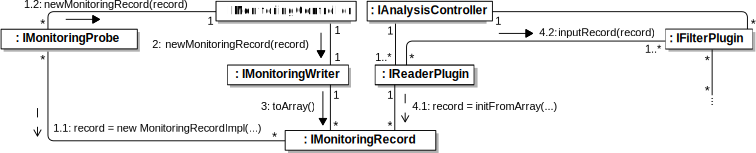
\includegraphics[width=1\textwidth]{images/kiekerCommunications-revisedReArranged-woMonitoringLog-bw-newNames}
\caption{Communication among \Kieker{} framework components}
\label{fig:KiekerCommunicationDiagram}
\end{figure}

% \vspace{1cm}

% Notify-tag because it is explained how Kieker works.
% avh: removed
\noindent The monitoring probes create the monitoring records containing the %
monitoring data and deliver them to the monitoring controller. %
The monitoring controller employs the monitoring writers to write these %
monitoring records to a monitoring log or stream. %
For analyzing purposes, monitoring reader plugins read the records from the %
monitoring log/stream. These records can then be further processed by a %
configuration of additional filter and repository plugins, inter-connected via input and output ports. %


\section{Kieker is Recommended by the SPEC Research Group}

In 2011, Kieker was reviewed and accepted for distribution as part of the SPEC Research %
Group's repository of peer-reviewed tools for quantitative system evaluation and analysis. %
See \url{http://research.spec.org/projects/tools.html} for details.


  \chapter{Quick Start Example}

This chapter provides a brief introduction to \Kieker{} based on a simple Bookstore example application. %
Section \ref{sec:example:downloadInstall} explains how to download and install \Kieker{}. The Bookstore application itself is introduced in Section \ref{sec:example:bookstore}, while the following Sections \ref{sec:example:monitoring} and \ref{sec:example:analysis} demonstrate how to use \Kieker{} for monitoring and analyzing the resulting monitoring data.

\section{Download and Installation}\label{sec:example:downloadInstall}

\Kieker{} can be downloaded from \KiekerURL. The web site provides zip/tar.gz archives of the \Kieker{} binary distribution as well as the corresponding \Kieker{} source code archives.

For this chapter, it is required to download and extract an archive containing \Kieker's binary distribution, e.g., \file{\binaryFileForDownload}. The extracted content has roughly the following directory structure:
% Note: The indention is not really necessary, but the tree is easier to understand in the tex-source.
\begin{figure}[H]
\begin{graybox}
\dirtree{%  
	.1 \KiekerDir/. 
		.2 bin/\DTcomment{Call scripts for \Kieker{} tools}. 
			.3 \ldots. 
		.2 doc/\DTcomment{}. 
			.3 tutorial/. 
				.4 userguide.pdf\DTcomment{PDF file of this document}. 
				.4 source-example/\DTcomment{Source code of the examples in this document}. 
		.2 dist/\DTcomment{The \Kieker{} framework libraries}. 
			.3 \analysisJar. 
			.3 \commonJar. 
			.3 \monitoringJar. 
			.3 \toolsJar. 
		.2 lib/\DTcomment{Libraries required by \Kieker{}}. 
			.3 \ldots. 
		.2 META-INF/\DTcomment{Example configuration files}. 
			.3 \ldots. 
}
\end{graybox}
\end{figure}

\section{A Simple Bookstore Application}\label{sec:example:bookstore}

The Bookstore application is a small sample application resembling a simple bookstore where a user can search for books in an online catalog.

Figure \ref{Figure:PlainBookstoreExample} shows the directory structure of the ``plain'' application neither with monitoring- nor with analysis-code.

\begin{figure}[H]
\begin{graybox}
\dirtree{%
.1 example/. %\DTcomment{The root directory of the project}.
.2 build/\DTcomment{Directory for the Java class files}. 
.2 src/\DTcomment{The directory for the source code files}.
.3 bookstoreApplication/.
.4 Bookstore.java.
.4 BookstoreStarter.java.
.4 Catalog.java.
.4 CRM.java.  
}
\end{graybox}

\caption{The directory structure of the Bookstore application}
\label{Figure:PlainBookstoreExample}
\end{figure}

The following listings show the content of the source code files:

\setJavaCodeListing
\lstinputlisting[caption=Bookstore.java]{source-example/plain-example/src/bookstoreApplication/Bookstore.java}
\lstinputlisting[caption=CRM.java]{source-example/plain-example/src/bookstoreApplication/CRM.java}
\lstinputlisting[caption=Catalog.java]{source-example/plain-example/src/bookstoreApplication/Catalog.java}
\lstinputlisting[caption=BookstoreStarter.java]{source-example/plain-example/src/bookstoreApplication/BookstoreStarter.java}

The example can be compiled and executed as follows:
\setBashListing
\begin{lstlisting}[caption=Compile and run under Linux]
> javac src/bookstoreApplication/*.java -d build

> java -classpath build bookstoreApplication.BookstoreStarter 
\end{lstlisting}

\warning The default command-line interpreter of Windows doesn't support automatic file expansion. Therefore every single sourcefile has to be passed:
\begin{lstlisting}[caption=Compile and run under Windows]
> javac src/bookstoreApplication/Bookstore.java 
        src/bookstoreApplication/BookstoreStarter.java 
        src/bookstoreApplication/Catalog.java 
        src/bookstoreApplication/CRM.java 
        -d build

> java -classpath build bookstoreApplication.BookstoreStarter 
\end{lstlisting}

Following listing shows an example run of the application:
\begin{lstlisting}[caption=Example run of the Bookstore application,label=lst:result-noinstr]
Bookstore.main: Starting request 0
Bookstore.main: Starting request 1
Bookstore.main: Starting request 2
Bookstore.main: Starting request 3
Bookstore.main: Starting request 4
\end{lstlisting}


\section{Monitoring}\label{sec:example:monitoring}
For the monitoring it is necessary to add some libraries from the \Kieker{}-framework to the example directory:
\begin{figure}[H]
\begin{graybox}
\dirtree{%
.1 example/. %\DTcomment{The root directory of the project}.
.2 build/\DTcomment{Directory for the Java class files}. 
.2 \newFilesDirTreeFormat lib/\DTcomment{Directory for the required libraries}.
.3 \newFilesDirTreeFormat \monitoringJar.
.3 \newFilesDirTreeFormat \commonJar.
.3 \newFilesDirTreeFormat \commonsLoggingJar.
.2 src/\DTcomment{The directory for the source code files}.
.3 \ldots.
}
\end{graybox}
\end{figure}

The \Kieker{} jar-files must be copied from the \dir{\KiekerDir/dist/} directory %
of the \Kieker{} release, as described in Section~\ref{sec:example:downloadInstall}. %
The file \file{commons-logging-1.1.1.jar} is included in \dir{\KiekerDir/lib/} %
and can also be copied from there.

The monitoring itself is done manually. Although this is not the strength of \Kieker\ it is pretty good for a quick start. Following listing shows how a method call is monitored:
\TODO{Imports?!}
% Make sure that this listing will be modified, once the sourcecode changes!!!
% It must show the whole monitoring of the bookstorecall, from getting the first time to persisting of the record!!
\setJavaCodeListing
\lstinputlisting[firstline=11, firstnumber=11, lastline=29, caption=Instrumentation of the \method{getBook()} call in Bookstore.java, label=listing:cuttingBookstore]%
{source-example/manual-monitoring/src/bookstoreApplication/Bookstore.java}
 
The time before and after a specific method call (in this case: \method{searchBook()}) is remembered. These information are stored in the so called operation execution record. Its (partially) layout can be seen in Figure \ref{Figure:OperationExecutionRecordClassDiagram}.

\begin{figure}[H]
\begin{centering}
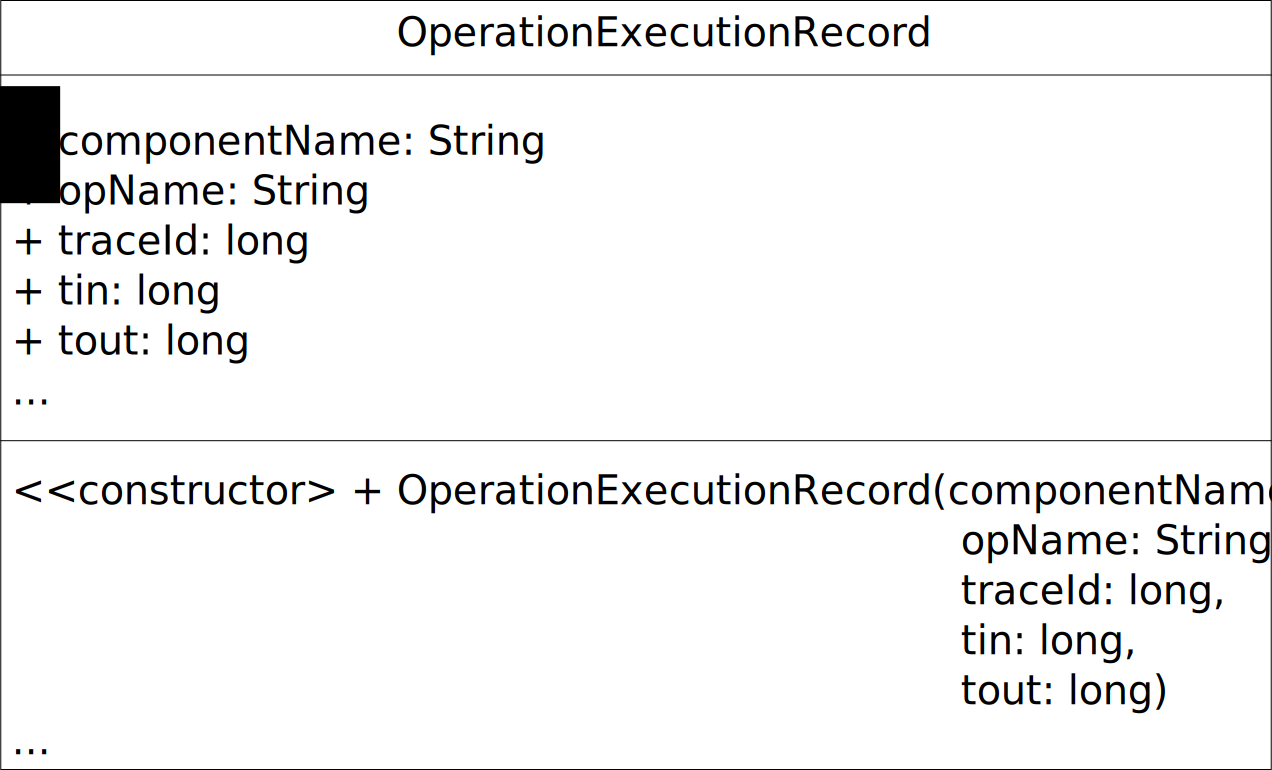
\includegraphics[width=0.4\textwidth]{images/OpExRecClassDiagram}
\caption{The class diagram of the operation execution record}
\label{Figure:OperationExecutionRecordClassDiagram}
\end{centering}
\end{figure}

The important attributes for now are:
\begin{itemize}
\item componentName: The component (the class) in which the called method is.
\item opName: The called method.
% \item traceId: The trace id of the current trace we want to record. Due to the fact, that we follow only one trace, this is zero in all recordings.
\item tin: The time before the source code which should be measured.
\item tout: The time after the source code which should be measured.
\end{itemize}

As an example another method in \file{CRM.java} is monitored as well:

\setJavaCodeListing
\lstinputlisting[firstline=16, firstnumber=16, lastline=27, caption=Instrumentation of the \method{getBook()} call in CRM.java, label=listing:cuttingCRM]%
{source-example/manual-monitoring/src/bookstoreApplication/CRM.java}
The instrumented example can now be compiled and executed as follows:

\setBashListing 		
\begin{lstlisting}[caption=Commands to compile and run the instrumented Bookstore under \UnixLikeSystems{},label=lst:bookstoreStarterLinux]
#\lstshellprompt{}# mkdir build
#\lstshellprompt{}# javac src/bookstoreApplication/*.java -classpath lib/#\mainJar# -d build/

#\lstshellprompt{}# java -classpath build/:
       lib/#\mainJar#:
       lib/#\commonsLoggingJar#
       bookstoreApplication.BookstoreStarter 
\end{lstlisting}
	
\warning Under Windows it is also necessary to seperate the different paths for the classpath with a semicolon instead of a colon.
\begin{lstlisting}[caption=Commands to compile and run the instrumented Bookstore under Windows,label=lst:bookstoreStarterWin]
#\lstshellprompt{}# mkdir build
#\lstshellprompt{}# javac src\kicker\examples\userguide\ch2bookstore\manual\*.java  
       -classpath lib\#\mainJar# -d build\

#\lstshellprompt{}# java -classpath build\;lib\#\mainJar#
       kicker.examples.userguide.ch2bookstore.manual.BookstoreStarter
\end{lstlisting}				

If everything worked correctly, there should now be a new directory with the %
name \dir{tpmon-20100727-181422131-UTC} (just with another timestamp) in the default %
temporary directory (under Linux this should be \dir{/tmp}; under Windows %
\dir{C:/temp}). In this directory, there should be a file with the extension %
\dir{.dat} which contains the recorded information from the source code and %
a file named \dir{tpmon.map} which contains information about the types of the %
monitoring records. %
The Listings~\ref{listing:exampledat} and \ref{listing:examplemap} show example %
contents. 
\begin{figure}[H]
\begin{graybox}
\dirtree{%
.1 /tmp/.
.2 tpmon-20100727-181422131-UTC/.
.3 tpmon.map.
.3 tpmon-20100727-181422234-UTC-Thread-2.dat.
}
\end{graybox}
\end{figure}

\setBashListing
\lstinputlisting[caption=tpmon-20100727-181422234-UTC-Thread-2.dat (excerpt), firstline=1, lastline=3, label=listing:exampledat]%
{ch2-quickstart-example/tpmon-20100727-181422131-UTC/tpmon-20100727-181422234-UTC-Thread-2.dat}

\lstinputlisting[caption=tpmon.map, label=listing:examplemap]%
{ch2-quickstart-example/tpmon-20100727-181422131-UTC/tpmon.map}

The \file{.dat}-file is saved as a CSV-file (\textbf{C}omma \textbf{S}eparated \textbf{V}alues), meaning that it can be opened with Microsoft Excel or OpenOffice.org Calc. It would be possible to visualize the stored data with the help of these programs, but we will show in Section \ref{sec:example:analysis} how to use \KiekerAnalysisPart\ to read and process the files.

\section{Analysis}\label{sec:example:analysis}
As mentioned in the beginning of this chapter, it is shown how a simple consumer is programmed before starting the analysis. Therefore we need some new files:
\begin{figure}[H]
\begin{graybox}
\dirtree{%  
.1 example/. 
.2 build/\DTcomment{Directory for the Java class files}. 
.2 lib/\DTcomment{Directory for the required libraries}.
.3 \ldots. 
.3 \newFilesDirTreeFormat \analysisJar.
.2 src/\DTcomment{The directory for the source code files}.
.3 bookstoreApplication.
.4 \ldots. 
.4 \newFilesDirTreeFormat BookstoreAnalysisStarter.java.
.4 \newFilesDirTreeFormat Consumer.java.
}
\end{graybox}
\end{figure}

The new jar-file can again be found in \dir{\KiekerDir/dist}. Listing \ref{listing:Consumer} shows the content of the new created \dir{Consumer.java}. It implements the \class{IMonitoringRecordConsumerPlugin} and overrides the necessary methods so that it can later be used by the analysis component of \Kieker. In this case the component gets a maximal response time within the constructor which will later be used to check whether a recorded method call replied fast enough or not. If the method call needed more time to response that the maximal allowed response time, it will be written directly to the error stream.\\
The methods \method{terminate} and \method{execute} don't do anything due to the fact that the consumer doesn't need any initialization. If the consumer would for example use threads then these methods would be the correct location to start and stop them.

\setJavaCodeListing       
\lstinputlisting[caption=Consumer.java, label=listing:Consumer]{source-example/manual-monitoring/src/bookstoreApplication/Consumer.java}

We have now to create the file \dir{BookstoreAnalysisStarter.java} to analyze our recorded information. 

\notify The analysis consists thereby of the following steps:
\begin{enumerate}
\item Create a new instance (or more) of the class \class{AnalysisInstance}.
\item Register the plugins which should evaluate the records.
\item Register exactly one reader to read the stored information.
\item Start the analysis instance.
\end{enumerate}

\setJavaCodeListing       
\lstinputlisting[caption=BookstoreAnalysisStarter.java]{source-example/manual-monitoring/src/bookstoreApplication/BookstoreAnalysisStarter.java}
As can be seen, the application expects the output directory from the earlier monitoring run (see Section \ref{sec:example:monitoring}) as argument, which must be passed manually. Following listings show again the course of action:
\setBashListing 		
\begin{lstlisting}[caption=Commands to compile and run the analysis under \UnixLikeSystems{},label=lst:bookstoreAnalysisStarterLinux] 			
#\lstshellprompt{}# mkdir build
#\lstshellprompt{}# javac src/bookstoreApplication/*.java
        -classpath lib/#\mainJar#
        -d build/

#\lstshellprompt{}# java -classpath
       build/:
       lib/#\mainJar#:
       lib/#\commonsLoggingJar#
       bookstoreApplication.BookstoreAnalysisStarter 
       /tmp/kieker-20110427-142244899-UTC-Kaapstad-KIEKER-SINGLETON
\end{lstlisting}	
	
\begin{lstlisting}[caption=Compile and run under Windows,label=lst:bookstoreAnalysisStarterWin] 			
#\lstshellprompt{}# javac src/bookstoreApplication/Bookstore.java 
        src/bookstoreApplication/BookstoreAnalysisStarter.java 
        src/bookstoreApplication/Catalog.java 
        src/bookstoreApplication/CRM.java 
        src/bookstoreApplication/Consumer.java
        -classpath
        lib/#\commonJar#:
        lib/#\monitoringJar#:
        lib/#\analysisJar#:
        -d build/

#\lstshellprompt{}# java -classpath 
       build/;
       lib/#\commonJar#;
       lib/#\monitoringJar#;
       lib/#\analysisJar#;
       lib/#\commonsLoggingJar#
       mySimpleKiekerExampleManual.BookstoreAnalysisStarter 
       C:\Temp\tpmon-20100808-092252697-UTC
\end{lstlisting}	
	
It should be ensured that the application gets the correct path from the monitoring run. 

If everything worked correctly, the consumer should write something on the outputstream for every record it gets. A possible display of the run can be found in the appendix of this tutorial. 
  %%%%%%%%%%%%%%%%%%%%%%%%%%%%%%%%%%%%%%%%%
% Kieker Monitoring Component
%
% $Date$
% $Rev$:
% $Author$


\chapter{\KiekerMonitoringPart{} Component}\label{chap:componentsMonitoring}

\NOTIFYBOX{The Java sources of this chapter, as well as a pre-compiled binary, %
can be found in the %
\file{\customComponentsBookstoreApplicationReleaseDirDistro{}/} directory of the %
binary release.}

\section{Monitoring Controller}\label{sec:componentsMonitoring:monitoringController}

\section{Monitoring Records}\label{sec:componentsMonitoring:monitoringRecords}

Monitoring records are objects that contain the monitoring data, as mentioned %
in the previous chapters. Typically, an instance of a monitoring record is %
constructed in a monitoring probe (Section~\ref{sec:monitoring:probe}), %
passed to the monitoring controller (Section~\ref{sec:componentsMonitoring:monitoringController}), %
serialized and deserialized by a monitoring %
writer (Section~\ref{sec:monitoring-log-writers}) and a
monitoring reader, and provided to analysis filters (Section~\ref{sec:analysis:controller}). %
Figure~\ref{fig:KiekerCommunicationDiagram} illustrates this life cycle of a monitoring %
record. %

In Chapter~\ref{chap:example}, we've already introduced and used the monitoring %
record type \class{OperationExecutionRecord}. \Kieker{} allows to use custom %
monitoring record types. Corresponding classes must implement the %
interface \class{IMonitoringRecord} shown in Figure~\ref{sec:monitoringrecord:interfacesAndImplementingClasses}. %
The methods \method{initFromArray}, \method{toArray}, \method{getValueTypes} %
are used for serialization and deserialization of the monitoring data contained %
in the record. Alternatively---in order to support the definition of immutable record types---the %
marker interface \class{IMonitoringRecord.Factory} needs to be implemented, requiring the %
implementation of (i)~the \method{toArray} method (as before), (ii)~a %
constructor accepting a values array, and (iii)~a public static \method{TYPES} %
field. The method \method{setLoggingTimestamp} is used by the monitoring controller to %
store the date and time when a record is received by the controller. %
The method \method{getLoggingTimestamp} can be used during analysis to retrieve %
this value. \KiekerMonitoringPart{} provides the abstract class %
\class{AbstractMonitoringRecord} (Figure~\ref{sec:monitoringrecord:interfacesAndImplementingClasses}) %
which already implements the methods to maintain the logging timestamp.

\begin{figure}[ht]\centering
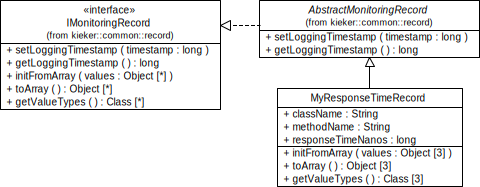
\includegraphics[scale=0.75]{images/kieker_MyRTRecord-modified}
\caption{Class diagram with the \class{IMonitoringRecord} and \class{IMonitoringRecord.Factory} interfaces, the abstract %
class \class{AbstractMonitoringRecord}, and a custom monitoring record type %
\class{MyResponseTimeRecord}}
\label{sec:monitoringrecord:interfacesAndImplementingClasses}
\end{figure}

%  \pagebreak

\noindent In order to use the abstract class for implementing your own monitoring record type, you need to:

\begin{enumerate}
\item Create a class that extends \class{AbstractMonitoringRecord}
\item  and
\begin{enumerate}
\item Override the methods \method{initFromArray}, \method{toArray}, \method{getValueTypes}
\item For immutable record types: implement \class{IMonitoringRecord.Factory}, a constructor %
with a single \class{Object[]} argument, and a public static \method{TYPES} field. %
In this case, \method{initFromArray} (which is not called by the framework then) should %
throw an \class{UnsupportedOperationException}.
\end{enumerate}
\end{enumerate}

\noindent The class \class{MyResponseTimeRecord}, shown in the class diagram in %
Figure~\ref{sec:monitoringrecord:interfacesAndImplementingClasses} and in %
Listing~\ref{listing:MyRecord}, is an example of a custom monitoring record type %
that can be used to monitor response times of method executions. %
Implementing \class{IMonitoringRecord.Factory}, \class{MyResponseTimeRecord} is %
an immutable type, i.e., it includes only final fields. %

\enlargethispage{1cm}

% \pagebreak 

\ % pushing the method initFromArray in the listing to the following page

\setJavaCodeListing
\lstinputlisting[caption=MyResponseTimeRecord.java, label=listing:MyRecord,firstline=27,firstnumber=27]{\customComponentsBookstoreApplicationDir/src/kieker/examples/userguide/ch3and4bookstore/MyResponseTimeRecord.java}

% \pagebreak

\section{Monitoring Probes}\label{sec:monitoring:probe}

The probes are responsible for collecting the monitoring data and passing it %
to the monitoring controller. %
In Chapter~\ref{sec:example:monitoring}, we have already demonstrated how to %
manually instrument a Java application. Listing~\ref{listing:cuttingBookstore} %
shows a similar manual monitoring probe, which uses the monitoring record type %
\class{MyResponseTimeRecord} defined in the previous Section~\ref{sec:componentsMonitoring:monitoringRecords}.

% Make sure that this listing will be modified, once the sourcecode changes!!!
% It must show the whole monitoring of the bookstorecall, from getting the first time to persisting of the record!!
% \pagebreak
\lstinputlisting[firstline=32, lastline=40, firstnumber=32, caption=Excerpt from Bookstore.java, label=listing:cuttingBookstore]{\customComponentsBookstoreApplicationDir/src/kieker/examples/userguide/ch3and4bookstore/Bookstore.java}

\noindent In order to avoid multiple calls to the \method{getInstance} method of the %
\class{MonitoringController} class, singleton instances should be stored %
in a final static variable, as shown in Listing~\ref{listing:cuttingBookstore:finalStaticController}.

\enlargethispage{1cm}

\lstinputlisting[firstline=24, lastline=25, firstnumber=24, caption=Singleton instance of the monitoring controller stored in a final static variable (excerpt from Bookstore.java), label=listing:cuttingBookstore:finalStaticController]{\customComponentsBookstoreApplicationDir/src/kieker/examples/userguide/ch3and4bookstore/Bookstore.java}

\noindent When manually instrumenting an application, the monitoring probe is implemented %
by mixing monitoring logic with business logic, which is often not desired since %
the resulting code is hardly maintainable. %
Many middleware technologies, such as Java~EE Servlet~\cite{JavaServletTechnology-WebSite}, %
Spring~\cite{Spring-WebSite}, and %
Apache~CXF~\cite{CXF-WebSite} provide interception/AOP~\cite{Kiczales1997} interfaces %
which are well-suited to implement monitoring probes. AspectJ~\cite{AspectJ-WebSite} allows to %
instrument Java applications without source code modifications. %
Chapter~\ref{chap:aspectJ} describes the \Kieker{} probes based on these technologies allowing to %
monitor trace information in distributed applications.

\section{Monitoring Writers}\label{sec:monitoring-log-writers}

Monitoring writers serialize monitoring records to the monitoring log/stream and  % and persist the recorded informations into files, databases etc. %
must implement the interface \class{IMonitoringWriter}. The monitoring %
controller passes the received records to the writer by calling the method %
\method{newMonitoringRecord}. Writers can use the methods to serialize the %
record contents, as described in Section~\ref{sec:componentsMonitoring:monitoringRecords}.

% This is the diagram with the hierarchy of the writers.
\begin{figure}[b]%[H]
	\begin{centering}
		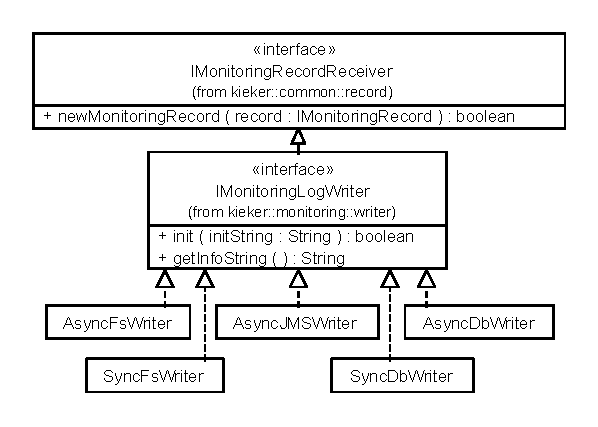
\includegraphics[scale=0.7]{images/kieker_writerimplsuserguide-modified}
		\caption{Interface \class{IMonitoringWriter} and some of the implementing classes}
		\label{figure:monitoringLogWritersHierarchy}
	\end{centering}
\end{figure}

Figure~\ref{figure:monitoringLogWritersHierarchy} shows some fo the monitoring writers %
already implemented in \KiekerMonitoringPart{}. The available properties for the %
included writers are well-documented in the %
example configuration file (see Appendix~\ref{sec:appdx:monitoringproperties}). %

% \enlargethispage{1.2cm}

Different writers can be used %
to store monitoring records to filesystems and databases respectively (e.g., \class{FileWriter}, \class{AsciiFileWriter}, %
\class{SyncFsWriter}, \class{AsyncDbWriter}, and \class{SyncDbWriter}). %
The variants with the prefix \class{Async} are implemented using asynchronous %
threads that decouple the I/O operations from the control flow of the %
instrumented application. %
As the new Kieker writer API uses always a fast pipe implementation to decouple the writer, nowadays all writers are asynchronuous.
Furthermore, the new \class{FileWriter} introduced new features and comes with a standard Kieker text serialization and a binary serialization.
In addition, it can be extended to write other formats.
The \class{AsciiFileWriter} is the default writer that has already been used in %
Section~\ref{sec:example:monitoring}. %
Please note that the database writers are currently in a prototype stage and
that they should be used with care. %
The \class{PrintStreamWriter} simply sends the String representation of incoming %
records to the standard output or standard error streams, which can be helpful %
for debugging purposes.

The \class{JmsWriter} and \class{JmxWriter} write records to a JMS %
(Java Messaging Service~\cite{JMS-WebSite}) queue and JMX (Java Management %
Extensions~\cite{JMX-Website}) queue respectively. The \class{PipeWriter} %
allows to pass records via in-memory record streams (named pipes). %
These writers allow to implement on-the-fly analysis in distributed systems, i.e., analysis while %
continuously receiving new monitoring data from an instrumented application potentially %
running on another machine. A more detailed description of how to use the \class{JmsWriter} %
can be found in Appendix~\ref{appendix:usingJMS}. %

\noindent Listing~\ref{listing:MyWriter} %on page~\pageref{listing:MyWriter} 
shows %
a custom writer \class{MyPipeWriter} which uses a named pipe to %
write the given records into a buffer located in the memory. The source code of %
the class \class{MyPipe} is listed in Appendix~\ref{appendix:pipeListings}. %

\setJavaCodeListing
\lstinputlisting[caption=MyPipeWriter.java, label=listing:MyWriter,firstline=23,firstnumber=23]{\customComponentsBookstoreApplicationDir/src/kieker/examples/userguide/ch3and4bookstore/MyPipeWriter.java}

% \pagebreak

\pagebreak

\noindent The monitoring writer to be used is selected by the %
\KiekerMonitoringPart{} configuration property (Section~\ref{chap:componentsMonitoring}) %
\textit{kieker.monitoring.writer}. Writer-specific configuration properties %
can be provided by properties prefixed by the fully-qualified writer classname.  %
Listing~\ref{lst:monitoringwriter:MyWriter} demonstrates how to use the custom %
writer \class{MyPipeWriter} defined above. In this example, the pipe name is %
passed as the property value \textit{pipeName}.

\setPropertiesListing
\lstinputlisting[caption={Configuration of the custom writer \class{MyPipeWriter}},label=lst:monitoringwriter:MyWriter,firstline=5,firstnumber=5,lastline=6]%
{\customComponentsBookstoreApplicationDir/src-resources/META-INF/kieker.monitoring.properties}

\enlargethispage{1cm}

\noindent As the data structure of this kind of monitoring stream, we created a %
class \class{PipeData} in order to demonstrate the use of the \method{toArray} and %
\method{initFromArray} (in Section~\ref{sec:analysis:reader}) methods. %
A \class{PipeData} object holds a logging timestamp and an \class{Object} array %
containing the serialized record data. %
Appendix~\ref{appendix:pipeListings} includes a source code listing of this class. %
Alternatively, we could have used \class{IMonitoringRecord} as the data structure %
used by the pipe. This is the way, \Kieker{}'s \class{PipeWriter} works. %

  %%%%%%%%%%%%%%%%%%%%%%%%%%%%%%%%%%%%%%%%%
% Kieker Analysis Component
% 
% $Date$
% $Rev$:
% $Author$


\chapter{\KiekerAnalysisPart{} Component}\label{chap:componentsAnalysis}

\NOTIFYBOX{The Java sources of this chapter can also be found in the %
\file{\customComponentsBookstoreApplicationDirDistro{}/} directory of the %
binary release.}

\section{Analysis Controller}\label{sec:analysis:controller}

An analysis with \KiekerAnalysisPart{} is set up and executed employing %
the class \class{AnalysisController}. %
\KiekerAnalysisPart{} requires a monitoring log reader %
(Section~\ref{sec:analysis:reader}) and at least %
one monitoring record consumer plugin (Section~\ref{sec:analysis:consumer}). %
In addition to the monitoring record consumer plugin, %
other analysis plugins can be registered. %
Figure~\ref{fig:analysisController:classdiagram} shows the class diagram %
with the important \KiekerAnalysisPart{} classes and their relationship. %

\begin{figure}[h]\centering
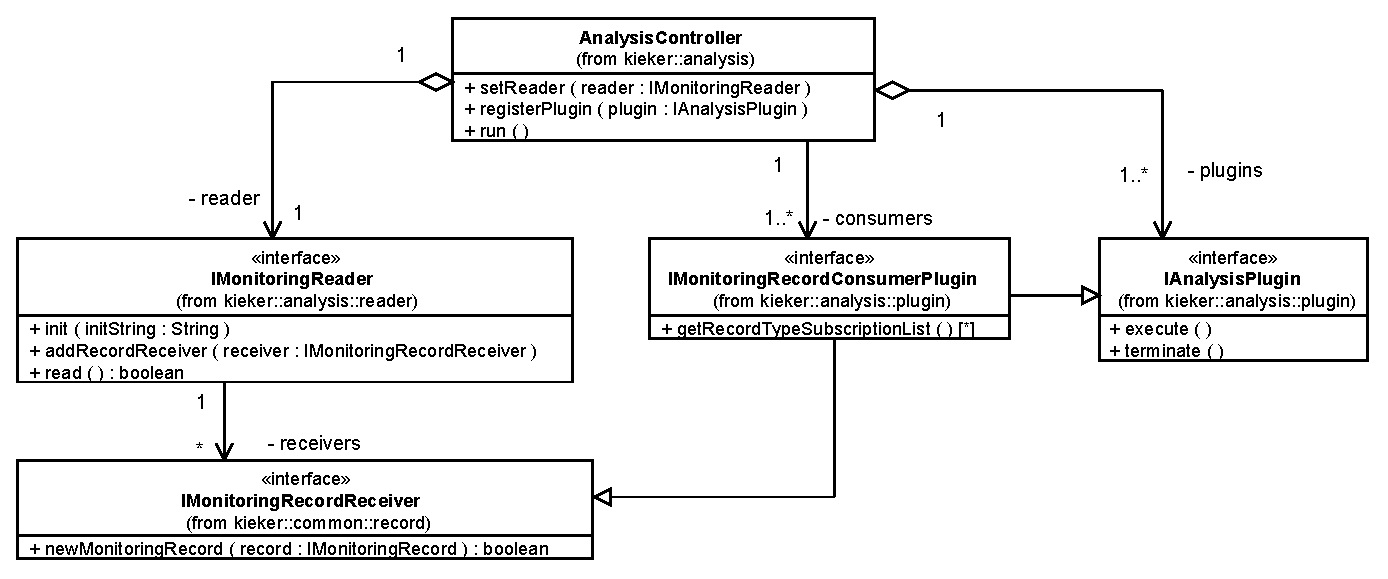
\includegraphics[scale=0.7]{images/kieker_AnalysisControlleruserguide-modified}
\caption{Class diagram showing important \KiekerAnalysisPart{} classes and their relationship}
\label{fig:analysisController:classdiagram}
\end{figure}

\noindent Setting up and running an analysis with \KiekerAnalysisPart{} requires the %
following steps to be performed, as described in Section~\ref{sec:example:analysis} already:\\

\begin{compactenum}
\item Creating an instance of the \class{AnalysisController} class
\item Creating and registering the monitoring log reader (\method{setLogReader}) as %
well as the monitoring record consumers and other analysis plugins (\method{registerPlugin}).
\item Starting the analysis instance (\method{run}).
\end{compactenum}

\

\noindent In the following Sections~\ref{sec:analysis:reader} and~\ref{sec:analysis:consumer}, %
we will create a custom monitoring log reader \class{MyPipeReader} and a %
monitoring record consumer plugin \class{MyResponseTimeConsumer}. %
\noindent The following Listing~\ref{listing:AnalysisController} shows how to create and run an analysis %
with these custom components:

\setJavaCodeListing
\lstinputlisting[caption=Code snippet setting up and running a \KiekerAnalysisPart{} instance (Starter.java),label=listing:AnalysisController,firstline=25, lastline=32, firstnumber=25]%
{\customComponentsBookstoreApplicationDir/src/bookstoreApplication/Starter.java}

\noindent On invocation of the \method{run} method, the \class{Analysis Controller} %
calls the \method{execute} if all analysis plugins allowing them to initialize. %
Then, it starts the configured monitoring log reader by calling its \method{read} %
method. Monitoring record consumers receive the monitoring records provided by %
the reader. As soon as the reader returns from the execution of its \method{read} 
method, the method \method{terminate} of each registered plugin is called by the %
\class{Analysis Controller}.

\section{Monitoring Log Readers}\label{sec:analysis:reader}

% Warning-tag for the reader-writer-thing
The monitoring log readers are the direct counterpart to the monitoring log %
writers. While writers receive records and write them into files or other kinds %
of monitoring logs, readers deserialize monitoring data and provide it as %
\class{IMonitoringRecord} instances. 

\begin{figure}\centering
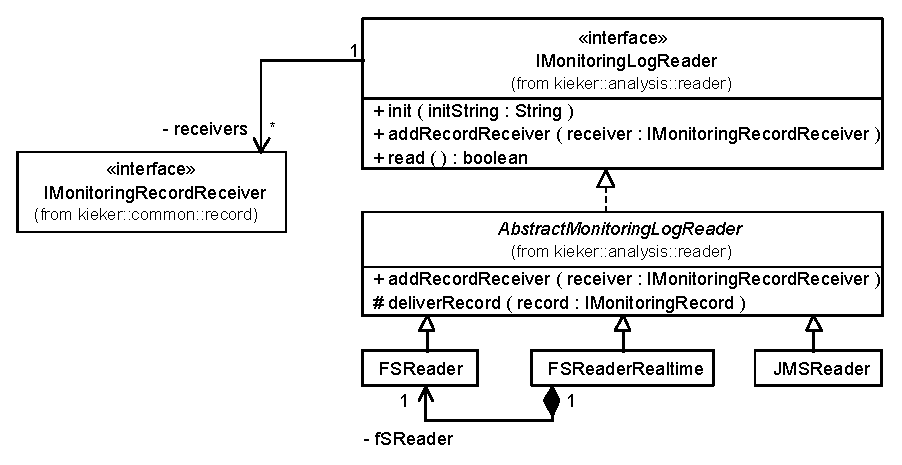
\includegraphics[scale=0.7]{images/kieker_readerimplsuserguide-modified}
\caption{Interface \class{IMonitoringLogReader} and implementing classes}
\label{Figure:ReaderHierarchy}
\end{figure}
% \
% 
% \WARNBOX{This means that whenever a new writer is implemented, a corresponding reader has to be implemented as well. If one want for example to store the recorded informations in a database, one should be capable of reading these saved informations from the database again.}
% 
% \

% \enlargethispage{1cm}

\noindent There are already some readers implemented in \Kieker\  as shown in the %
class diagram in Figure \ref{Figure:ReaderHierarchy}. %
The \class{FSReader} has already been used in Section~\ref{sec:example:analysis}. %
The \class{FSReaderRealtime} can be used to simulate continuous monitoring of a %
production system. It adds delays between the delivery of the monitoring records %
to its consumers according to the original delays reconstructed from the logging %
timestamps (Section~\ref{sec:componentsMonitoring:monitoringRecords}).
A brief description of how to use the \class{JMSReader} can be found in Appendix~\ref{appendix:usingJMS}. %

\noindent The implementation of a custom reader is similar to implementating a %
monitoring log writer. Custom reader should extend the class \class{AbstractKiekerMonitoringLogReader} %
which already provides an implementation of the observer pattern. %
By invoking the method \method{deliverRecord},  the delivery of records is then %
delegated to the super class.

Listing~\ref{listing:MyReader} shows a simple reader which polls records from %
the named pipe introduced in the previous Chapter~\ref{chap:componentsMonitoring}. %

% If there is nothing on the pipe to be read, the reader waits 4 seconds at maximum before it terminates.

\setJavaCodeListing
\lstinputlisting[caption=MyPipeReader.java, label=listing:MyReader,float]{\customComponentsBookstoreApplicationDir/src/bookstoreApplication/MyPipeReader.java}

\section{Analysis Plugins}\label{sec:analysis:plugins}

Any analysis or visualization component used with \KiekerAnalysisPart{} must %
implement the interface \class{IAnalysisPlugin} (Figure~\ref{fig:analysisController:classdiagram}). %
As described in Section~\ref{sec:analysis:controller}, the life-cycle of each %
registered plugin is controlled by the \class{Analysis Controller} instance %
employing the methods \method{execute} and \method{terminate}. Analysis plugins %
must implement these methods for initialization and termination.

The monitoring record consumer plugins described in the following %
Section~\ref{sec:analysis:consumer}, are special analysis plugins that receive %
the monitoring records provided by the monitoring log reader. %
Starting with these monitoring record plugins, analysis plugins can be connected %
in a pipe-and-filter style to implement more complex analyses. %
\Kieker{} provides input and output port interface and implementing classes %
to implement such analyses. See the documentation of the classes \class{AbstractInputPort} %
and \class{OutputPort} for details. \KiekerTraceAnalysis{} is implemented %
based on this pattern. 

\section{Monitoring Record Consumer Plugins}\label{sec:analysis:consumer}

As just mentioned, consumer plugins are special analysis plugins which receive %
the records provided by the monitoring log reader and implement analyses or %
visualizations based on these records. %
Consumer plugins must implement the interface \class{IMonitoringRecordConsumerPlugin} %
(see Figure~\ref{fig:analysisController:classdiagram}). %
By implementing the \method{getRecordTypeSubscriptionList} method, a consumer plugin %
can specify the desired types of monitoring records to be received via the %
method \method{newMonitoringRecord}.


The custom consumer in Listing~\ref{lst:MyReponseTimeConsumer} simply writes %
the content of the received response time records to the standard output stream.

\setJavaCodeListing
\lstinputlisting[caption=MyReponseTimeConsumer.java,label=lst:MyReponseTimeConsumer]{\customComponentsBookstoreApplicationDir/src/bookstoreApplication/MyResponseTimeConsumer.java}

  \chapter{Trace Analysis and Monitoring via AspectJ}\label{chap:aspectJ}

This chapter will show in Section \ref{sec:aspectJ:annotation} how
to use AspectJ to mark methods to be monitored with a simple annotation
in order to avoid the manual monitoring as seen in Chapter \ref{chap:example}
and \ref{chap:componentsMonitoring}. Once the methods are marked, the AspectJ-Weaver-Agent
will surround the calls with the necessary code during runtime, similar
to the hardcoded code used in Section \ref{sec:example:monitoring}.
An alternative solution will be shown as well in Section \ref{sec:aspectJ:fullweaving}
in which everything will be monitored - without exceptions. Both solutions
can be used to reconstruct the architecture and to perform a trace
analysis. The result of both will be diagrams similar to Figure \ref{fig:bookstore:classAndSequenceDiagrams}.

The idea of weaving the monitoring-code into the ``plain'' code
during compile-time seems to suggest itself, but in this chapter it
is only shown how to perform the so called load-time-weaving - the
weaving during runtime, which is way more flexible than the compile-time-weaving.

\section{AspectJ Annotations}\label{sec:aspectJ:annotation}

To weave the code via AspectJ with the \Kieker{}-Framework,
some new files are required, including the AspectJ-Agent and a configuration
file for AspectJ. Following figure shows the resulting directory tree
with the necessary files, based on the BookstoreApplication shown
in Chapter \ref{chap:example}.

\begin{figure}[H]
\begin{graybox}
\dirtree{%
.1 \DirInDirTree{example/}. %\DTcomment{The root directory of the project}.
.2 \DirInDirTree{build/}\DTcomment{Directory for the Java class files}.
.2 \DirInDirTree{META-INF/} \DTcomment{Directory for the configuration files}.
.3 \aopConfigFile. 
.2 \DirInDirTree{lib/} \DTcomment{Directory for the needed libraries}.
.3 \monitoringJar.
.3 \commonJar.
.3 \commonsLoggingJar.
.3 \aspectJWeaverJar.  
.2 \DirInDirTree{src/}\DTcomment{Directory for the source code files}.
.3 \DirInDirTree{bookstoreApplication/}.
.4 Bookstore.java.
.4 BookstoreStarter.java.
.4 Catalog.java.
.4 CRM.java.  
}
\end{graybox}

\caption{The new directory structure of the Bookstore application}
\end{figure}

The new jar-file \file{aspectjweaver-1.6.9.jar} can again be found
in the \dir{lib}-dir from the \Kieker{}-binaries, as well as the
configuration file \file{\aopConfigFile} can be found in the directory \dir{META-INF}.

Once the necessary file has been copied to the example-directory,
the sourcecode can be instrumented with the annotation \class{OperationExecutionMonitoringProbe}.
Listing \ref{listing:BookstoreAspectJ} shows how the annotation is
used.

\setJavaCodeListing
\lstinputlisting[caption=Bookstore.java, label=listing:BookstoreAspectJ]{\aspectJBookstoreApplicationDir/src/bookstoreTracing/Bookstore.java}

As an example all methods within the four sourcecode-files will be
annotated. It is possible to mark nearly every method with the annotation
- except constructors.
\TODO{Something is missing, I know...}
\section{Full Monitoring}\label{sec:aspectJ:fullweaving}
\TODO{Still missing something...}

  
  % suppress appendix chapters in toc
  %%%%%%%%%%%%%%%%%%%%%%%%%%%%%%%%%%%%%%%%%
% Appendix
% 
% $Date$
% $Rev$:
% $Author$


\appendix

\chapter*{Appendix}\label{appendix}
\addcontentsline{toc}{chapter}{Appendix}
\addtocontents{toc}{\protect\setcounter{tocdepth}{-1}}

\chapter{Wrapper scripts}\label{appendix:wrapperScripts}
The \dir{bin/} directory of \Kieker's binary release contains some \file{.sh}  and %
\file{.bat} scripts to invoke tools included in \file{\mainJar{}}. %
The following sections give a short description of their functionality and %
list their usage outputs as printed to the standard output stream when %
called without command-line parameters. %
In addition to the standard output stream, the file \file{kieker.log} %
is used for logging output during execution.

% generated by the script gen-bin-usage-tex.sh with manual adjustments

\section{Script \file{convertLoggingTimestamp.sh|bat}}

The script converts \KiekerMonitoringPart{} logging timestamps, %
representing the number of nanoseconds since 1~Jan 1970 00:00 UTC, to a %
human-readable textual representation. %

\

\noindent Main-class: {\small \class{kieker.tools.loggingTimestampConverter.LoggingTimestampConverterTool}}

\paragraph*{Usage}\

\setTextListing
\lstinputlisting[caption=]{Appendix-usage-convertLoggingTimestamp.sh.inc}

\paragraph*{Example}\

\setTextListing
\begin{lstlisting}
$\lstshellprompt{}$ $\textbf{bin/convertLoggingTimestamp.sh}$ $\textbf{-t}$ 1283156545581511026 1283156546127117246 
1283156545581511026: Mo, 30 Aug 2010 08:22:25 +0000 (UTC) (Mo, 30 Aug 2010 10:22:25 +0200 (local time))
1283156546127117246: Mo, 30 Aug 2010 08:22:26 +0000 (UTC) (Mo, 30 Aug 2010 10:22:26 +0200 (local time))
\end{lstlisting}

\section{Script \file{logReplay.sh|bat}}

Replays filesystem monitoring logs created by \KiekerMonitoringPart{}. %
Example applications are:
\begin{compactitem}
\item Merging multiple directories containing monitoring data into a single %
output directory. 
\item Importing a filesystem monitoring log to another monitoring log, e.g., %
a database. Therefore, an appropriate \KiekerMonitoringPart{} configuration %
file must be passed to the script (see Section~\ref{sec:monitoring:configuration}).
\item Replaying a recorded filesystem monitoring log in real-time in order to simulate %
incoming monitoring data from a running system, e.g., via JMS~(see also Appendix~\ref{appendix:usingJMS}). 
\end{compactitem}

\

\noindent Main-class: {\small \class{kieker.tools.logReplayer.FilesystemLogReplayerStarter}}

\paragraph*{Usage}\

\setTextListing
\lstinputlisting[caption=]{Appendix-usage-logReplay.sh.inc}

\paragraph*{Example}\

\noindent The following command replays the monitoring testdata included in %
the binary release to another directory:

\setTextListing
\begin{lstlisting}
$\lstshellprompt{}$ $\textbf{bin/logReplay.sh}$
  $\textbf{--inputdirs}$ $\distributedTestdataDirDistro$ 
  $\textbf{--keep-logging-timestamps}$ $true$ 
  $\textbf{--realtime}$ $false$
\end{lstlisting}

\section{Script \file{trace-analysis.sh|bat}}

\paragraph*{Usage}\

\setTextListing
\lstinputlisting[caption=]{Appendix-usage-trace-analysis.sh.inc}

\paragraph*{Example}\

Examples on using this script can be found in Chapter~\ref{chap:aspectJ} and %
Appendix~\ref{appendix:traceAnalysisOutputExamples}.

\chapter{\KiekerMonitoringPart{} Configuration File}\label{sec:appdx:monitoringproperties}

This is the file \file{\monitoringPropertiesFile} from the binary release and 
constitutes \KiekerMonitoringPart{}'s default configuration.

\

\setXMLListing
\lstinputlisting[caption=\monitoringPropertiesFile]{../../META-INF/kieker.monitoring.properties}

\section{Script \file{dotPic-fileConverter.sh|bat}}

\paragraph*{Usage \& Example}\

\setTextListing
\lstinputlisting[caption=,firstline=3]{Appendix-usage-dotPic-fileConverter.sh.inc}



\chapter{\KiekerMonitoringPart{} Default Configuration}\label{sec:appdx:monitoringproperties}
This is the file \file{\monitoringPropertiesFile} from the binary release and 
constitutes \KickerMonitoringPart{}'s default configuration. %
Section~\ref{sec:monitoring:configuration} describes how to use a custom configuration.

\

\setPropertiesListing
\lstinputlisting[caption=\monitoringPropertiesFile]{../../src/monitoring/META-INF/kicker.monitoring.default.properties}


\chapter{Additional Source Code Listings}\label{appendix:additionalSourceCode}
\section{MyNamedPipeManager and MyPipe}\label{appendix:pipeListings}

\enlargethispage{1cm}

      \setJavaCodeListing
      \lstinputlisting[firstline=21, firstnumber=21,caption=MyNamedPipeManager.java]{\customComponentsBookstoreApplicationDir/src/bookstoreApplication/MyNamedPipeManager.java}
\newpage
      \setJavaCodeListing
      \lstinputlisting[firstline=21, firstnumber=21, caption=MyPipe.java]{\customComponentsBookstoreApplicationDir/src/bookstoreApplication/MyPipe.java}
      
      \setJavaCodeListing
      \lstinputlisting[firstline=21, firstnumber=21, caption=PipeData.java]{\customComponentsBookstoreApplicationDir/src/bookstoreApplication/PipeData.java}

\chapter{Example Console Outputs}\label{appendix:exampleConsoleOutputs}
\section{Quick Start Example (Chapter~\ref{chap:example})}\label{sec:appendix:manualInstrumentation:output}
% \subsubsection{Monitoring}
% 		The following listing shows the produced log during a run of the Bookstore Application with the manual monitoring probes.
\setTextListing
\lstinputlisting[caption=Execution of the manually instrumented Bookstore application (Section~\ref{sec:example:monitoring})]
{ch2-quickstart-example/kieker-20120402-163314855-UTC-myHost-KIEKER-SINGLETON-monitoring.stdout}
\newpage
% \subsubsection{Analysis}
% 		The second listing is the log during the analysis of the produced data. It can be seen that some of the calls are accepted and some others refused.
\setTextListing
\lstinputlisting[caption=Execution of the example analysis (Section~\ref{sec:example:analysis})]
{ch2-quickstart-example/kieker-20130910-120352847-UTC-myHost-KIEKER-SINGLETON-analysis.stdout}
\newpage	
\section{Trace Monitoring, Analysis \& Visualization (Chapter \ref{chap:aspectJ})}%
\label{sec:appendix:exampleConsoleOutputs:aspectJExample}
\setTextListing
\begin{lstlisting}[caption=Execution of the Bookstore with AspectJ trace instrumentation (Section~\ref{sec:traceAnalysis:instr:AspectJ})]
Bookstore.main: Starting request 0
10.04.2012 13:03:51 kieker.monitoring.core.configuration.ConfigurationFactory createSingletonConfiguration
INFO: Loading properties from properties file in classpath: 'META-INF/kieker.monitoring.properties'
10.04.2012 13:03:51 kieker.monitoring.core.controller.MonitoringController createInstance
INFO: Current State of kieker.monitoring (1.5) Status: 'enabled'
        Name: 'KIEKER'; Hostname: 'pc-vanhoorn'; experimentID: '1'
JMXController: JMX disabled
RegistryController: 0 strings registered.
TimeSource: 'kieker.monitoring.timer.SystemNanoTimer'
        Time in nanoseconds (with nanoseconds precision) since Thu Jan 01 01:00:00 CET 1970'
WriterController:
        Number of Inserts: '0'
        Automatic assignment of logging timestamps: 'true'
Writer: 'kieker.monitoring.writer.filesystem.AsyncFsWriter'
        Configuration:
                kieker.monitoring.writer.filesystem.AsyncFsWriter.QueueFullBehavior='0'
                kieker.monitoring.writer.filesystem.AsyncFsWriter.flush='true'
                kieker.monitoring.writer.filesystem.AsyncFsWriter.QueueSize='10000'
                kieker.monitoring.writer.filesystem.AsyncFsWriter.customStoragePath='.'
                kieker.monitoring.writer.filesystem.AsyncFsWriter.MaxShutdownDelay='-1'
                kieker.monitoring.writer.filesystem.AsyncFsWriter.storeInJavaIoTmpdir='true'
                kieker.monitoring.writer.filesystem.AsyncFsWriter.maxEntriesInFile='25000'
        Records lost: 0
        Writer Threads (1): 
                Finished: 'false'; Writing to Directory: '/tmp/kieker-20110428-142829399-UTC-Kaapstad-KIEKER'
Sampling Controller: Periodic Sensor available: Current Poolsize: '0'; Scheduled Tasks: '0'

10.04.2012 13:03:51 kieker.monitoring.core.registry.ControlFlowRegistry <clinit>
INFO: First threadId will be 7752665283541598209
10.04.2012 13:03:51 kieker.monitoring.core.controller.MonitoringController$\$$1 run
INFO: ShutdownHook notifies controller to initiate shutdown
10.04.2012 13:03:51 kieker.monitoring.core.controller.MonitoringController cleanup
INFO: Shutting down Monitoring Controller (KIEKER)
10.04.2012 13:03:51 kieker.monitoring.writer.AbstractAsyncWriter terminate
INFO: Shutting down writers.
\end{lstlisting}




\chapter{Ant Scripts}\label{appendix:antScripts}
\section{Quick Start Example (Chapter \ref{chap:example})}
The following \file{build.xml} and \file{build.properties} files can be %
used for compiling and executing the manually instrumentated Bookstore %
application and the analysis, as described in Chapter~\ref{chap:example}. %
The files are included in the directory \file{\manualInstrumentedBookstoreApplicationDirDistro{}/}.

      In order to run the analysis of the application, it is necessary to pass the location of the monitoring log directory. This is done via the parameter \textit{analysis.directory}, e.g.:
      \setBashListing
      \begin{lstlisting}[caption=Command to compile and run the instrumented Bookstore via ant]
#\lstshellprompt{}# ant run-analysis -Danalysis.directory /tmp/kieker-20120402-163314855-UTC-myHost-KIEKER-SINGLETON
\end{lstlisting}%-KIEKER


% \enlargethispage{1.2cm}
      \setPropertiesListing
      \lstinputlisting[caption=build.properties]{\manualInstrumentedBookstoreApplicationDir/build.properties}
      \setAntListing
      \lstinputlisting[caption=build.xml]{\manualInstrumentedBookstoreApplicationDir/build.xml}
\newpage
\section{Custom Components (Chapters \ref{chap:componentsMonitoring} and \ref{chap:componentsAnalysis})}
      The following \file{build.xml} and \file{build.properties} files can be used for compiling and executing the manually instrumentated Bookstore application with the custom components, as described in Chapters~\ref{chap:componentsMonitoring} and \ref{chap:componentsAnalysis}. %
The files are included in the directory \file{\customComponentsBookstoreApplicationDirDistro{}/}.
      \setPropertiesListing
      \lstinputlisting[caption=build.properties]{\customComponentsBookstoreApplicationDir/build.properties}
      \setAntListing
      \lstinputlisting[caption=build.xml]{\customComponentsBookstoreApplicationDir/build.xml}
\newpage
\section{AspectJ-based Trace Monitoring (Chapter \ref{chap:aspectJ})}
      The following \file{build.xml} and \file{build.properties} files can be used for compiling and executing the Bookstore application instrumentated with AspectJ (see Chapter~\ref{chap:aspectJ}). %
The files are included in the directory \file{\aspectJBookstoreApplicationDirDistro{}/}.
\vspace{-3ex}
      \setPropertiesListing
      \lstinputlisting[caption=build.properties]{\aspectJBookstoreApplicationDir/build.properties}     
\enlargethispage{1.1cm}
      \setAntListing
      \lstinputlisting[caption=build.xml]{\aspectJBookstoreApplicationDir/build.xml}

\chapter{Java~EE Servlet Container Example}\label{appendix:JavaEEServletExample}
The \Kieker{} download site\footnote{\KiekerDownloadURL{}} includes an additional %
example \file{\JavaEEServletExampleName}. Using the sample Java Web application %
iBATIS JPetStore\footnote{\url{http://ibatis.apache.org/}}, this example %
demonstrates how to employ \KiekerMonitoringPart{} for monitoring a Java application %
running in a Java~EE container---in this case, Apache Tomcat\footnote{\url{http://tomcat.apache.org/}}. %
Monitoring probes based on the Java~EE Servlet API %
and AspectJ are used to monitor execution, trace, and session data (see Section~\ref{chap:aspectJ}).

\section{Preparation of the Tomcat Servlet Container}

\begin{compactenum}
\item Copy the files \file{\mainJar}, \file{\commonsLoggingJar}, and \file{\aspectJWeaverJar} from %
\Kieker{}'s binary distribution to the Tomcat's \dir{lib/} directory.
\item Copy the file \file{\servletWar} from \Kieker{}'s %
binary distribution to the Tomcat's \dir{webapps/} directory.
\item Tomcat's \dir{lib/} directory contains the files \file{kieker.monitoring.properties} %
and \file{aop.xml} --- the configuration of \KiekerMonitoringPart{} and the %
AspectJ-based instrumentation. %
\item
 Tomcat's start script \file{bin/catalina.\{sh|bat\}} file was modified to add the location %
of the \file{kieker.\-moni\-toring.properties} and the AspectJ agent to the argument %
list of the JVM call:
\end{compactenum}

\enlargethispage{1cm}

\setPropertiesListing
\lstinputlisting[firstline=188,firstnumber=188,lastline=190,caption={Excerpt from catalina.sh (for \UnixLikeSystems)},numbers=left]{\JavaEEServletExampleDir/Tomcat6.0.18WithJpetStore-withInstrumentedJPetStore/bin/catalina.sh}

\setPropertiesListing
\lstinputlisting[firstline=121,firstnumber=121,lastline=123,caption={Excerpt from catalina.bat (for Windows)},numbers=left]{\JavaEEServletExampleDir/Tomcat6.0.18WithJpetStore-withInstrumentedJPetStore/bin/catalina.bat}

%% BEGIN: Windoof
% set JAVA_HOME=%ProgramFiles%\Java\jdk1.6.0_23
% start bin/startup.bat
%% END: Windoof

\begin{compactenum}\setcounter{enumi}{4}
\item  A prepared \file{jpetstore.war} file is already located in the %
   Tomcat's \dir{webapps/} directory. If you want to rebuild the sources, %
   for example to modify the instrumentation, see Section~\ref{sec:Appendix:JPetStoreExample:rebuild}. 
\end{compactenum}


\section{JPetStore and \KiekerMonitoringPart{} Control Servlet}

\noindent We will now start the Tomcat server and generate some monitoring data by manually %
accessing the JPetStore web application. 

\

\enlargethispage{1.5cm}

\begin{compactenum}
\item Start the Tomcat server using the \file{bin/startup.sh} or \file{bin/startup.bat} (\UnixLikeSystems/Windows) %
   script in the Tomcat's \dir{bin/} directory.

   You should make sure, that the Tomcat started properly, by taking 
   a look at the \file{logs/catalina.out} file, \file{logs/catalina.<date>.log} file respectively. %
   On error, the file \file{logs/localhost.<date>.log} may contain details % 
   to resolve the issue.
\item Now, you can access the JPetStore application by opening the URL
   \url{http://localhost:8080/jpetstore/} (Figure~\ref{fig:jpetstore}). %
   \Kieker{} intialization messages should appear in \file{logs/catalina.out}, \file{logs/catalina.<date>.log} respectively. %
   The output includes the information where the monitoring data is written to
   (should be Tomcat's \dir{temp/kieker-<DATE-TIME>/} directory).
\item  Browse through the application to generate some monitoring data. %
   This data can be analyzed and visualized using \KiekerTraceAnalysis{}, %
   as described in Chapter~\ref{chap:aspectJ}.
\item \Kieker{} includes a servlet to control the status of \KiekerMonitoringPart{}. %
   It can be accessed via \url{http://localhost:8080/kieker-monitoring-servlet-\version/} %
   (Figure~\ref{fig:controlServlet}).
\end{compactenum}

\begin{figure}[h]\centering
\hfill
\subfigure[iBATIS JPetStore]{\label{fig:jpetstore}%
\includegraphics[width=0.45\textwidth]{images/jpetstore-example-FFscrsh}}
\hfill
\subfigure[\KiekerMonitoringPart{} control servlet]{\label{fig:controlServlet}%
\includegraphics[width=0.45\textwidth]{images/kieker-servlet-FFscrsh-version-obfuscated}}
\hfill
\caption{}
\end{figure}

\newpage

\section{Rebuilding the JPetStore Application}\label{sec:Appendix:JPetStoreExample:rebuild}

\noindent In order to rebuild the JPetStore sources (located in \dir{JPetStore-5.0-instrumented/}), 
the following steps are required:

\

\begin{compactenum}
\item Copy the \file{\mainJar{}} from \Kieker{}'s
   binary distribution to the JPetStore's \dir{devlib/} directory. %
   It is required for the annotation-based instrumentation %
   (\texttt{@Ope\-rationExecutionMonitoringProbe}), as described in Chapter~\ref{chap:aspectJ}
\item Build the JPetStore with the \file{build.xml} by calling \texttt{ant} from %
    within \dir{build/} directory. 
\item You'll find the packaged JPetStore \file{.war}-file in \dir{build/wars/}.
\item Copy the file to the Tomcat's \dir{webapps/} directory.
\end{compactenum}



\chapter{Using the JMS Writer and Reader}\label{appendix:usingJMS}
This chapter gives a brief description on how to use the \class{AsyncJmsWriter} and \class{JmsReader} %
classes. The directory \dir{\JMSBookstoreApplicationReleaseDirDistro/} contains the %
sources, gradle scripts etc.\ used in this example. It is based on the Bookstore %
application with manual instrumentation presented in Chapter~\ref{chap:example}. %

The following sections provide step-by-step instructions for the %
ActiveMQ JMS server implementation (Section~\ref{example:jms:activemq}).
The general procedure for this example is the following:

\medskip

\begin{compactenum}
 \item Download and prepare the respective JMS server implementation
 \item Copy required libraries to the example directory
 \item Start the JMS server
 \item Start the analysis instance which receives records via JMS
 \item Start the monitoring instance which sends records via JMS
\end{compactenum}

\

\WARNBOX{\quad\\Due to a bug in some JMS servers, avoid paths including white spaces.}

\section{ActiveMQ}\label{example:jms:activemq}

\subsection{Download and Prepare ActiveMQ}

Download an ActiveMQ archive from \url{http://activemq.apache.org/download.html}
and decompress it to the base directory of the example. Note, that there are two different %
distributions, one for Unix/Linux/Cygwin and another one for Windows, and that the latest supported version of ActiveMQ compatible with Java 7 is 5.14.5. 

Under \UnixLikeSystems{}, you'll need to set the executable-bit of the start script:

\setBashListing
\begin{lstlisting}[caption=]
 #\lstshellprompt{}# chmod +x bin/activemq
\end{lstlisting}

\noindent Also under \UnixLikeSystems{}, make sure that the file \file{bin/activemq} %
includes UNIX line endings (e.g., using your favorite editor or the \textit{dos2unix} tool).

\subsection{Copy ActiveMQ Libraries}

Copy the following files from the ActiveMQ release to the %
\dir{lib/} directory of this example:

\medskip

\enlargethispage{0.5cm}

\begin{compactenum}
\item \file{activemq-all-<version>.jar} (from ActiveMQ's base directory)
\item \file{slf4j-log4j<version>.jar} (from ActiveMQ's \dir{lib/optional} directory)
\item \file{log4j-<version>.jar} (from ActiveMQ's \dir{lib/optional} directory)
\end{compactenum}

\subsection{Kieker Monitoring Configuration for ActiveMQ}

The file \file{src-resources/META-INF/kieker.\-monitoring.\-pro\-perties-activeMQ} %
is already configured to use the \class{JmsWriter} via ActiveMQ. The important properties are %
the definition of the provider URL and the context factory:

\setPropertiesListing
\lstinputlisting[firstline=12,lastline=12,caption=Excerpt from \file{kieker.monitoring.properties-activemq} configuring the provider URL of the JMS writer via ActiveMQ]{\JMSBookstoreApplicationDir/src-resources/META-INF/kieker.monitoring.properties-activemq}

\setPropertiesListing
\lstinputlisting[firstline=21,lastline=21,caption=Excerpt from \file{kieker.monitoring.properties-activemq} configuring the context factory of the JMS writer via ActiveMQ]{\JMSBookstoreApplicationDir/src-resources/META-INF/kieker.monitoring.properties-activemq}

\subsection{Running the Example}

% \paragraph*{Execution}%
 The execution of the example is performed by the following three steps:
\begin{enumerate}
\item Start the JMS server (you may have to set your \class{JAVA\_HOME} variable first):

\setBashListing
\begin{lstlisting}[caption=Start of the JMS server under UNIX-like systems]
#\lstshellprompt{}# bin/activemq start
\end{lstlisting}
\begin{lstlisting}[caption=Start of the JMS server under Windows]
#\lstshellprompt{}# bin\#activemq start
\end{lstlisting}
\item Start the analysis part (in a new terminal):
\setBashListing
\begin{lstlisting}[caption=Start the analysis part under UNIX-like systems]
#\lstshellprompt{}# ./gradlew runAnalysisActiveMQ
\end{lstlisting}
\begin{lstlisting}[caption=Start the analysis part under Windows]
#\lstshellprompt{}# gradlew.bat runAnalysisActiveMQ
\end{lstlisting}
\item Start the instrumented Bookstore (in a new terminal):
\setBashListing
\begin{lstlisting}[caption=Start the analysis part under UNIX-like systems]
#\lstshellprompt{}# ./gradlew runMonitoringActiveMQ
\end{lstlisting}
\begin{lstlisting}[caption=Start the analysis part under Windows]
#\lstshellprompt{}# gradlew.bat runMonitoringActiveMQ
\end{lstlisting}
\end{enumerate}


\chapter{Libraries}\label{appendix:libraries}
    The following table shows all libraries which are used by \Kieker\ and explains them briefly. %
These libraries are included in the \dir{lib/} directory of both the \Kieker{} binary and %
source distributions.

The Apache Commons~\cite{CommonsLogging-WebSite} library (\file{\commonsLoggingJar}) %
is the only third-party library always needed when using \Kieker{}. %
The need to provide the additional libraries in the classpath depends on the %
specific configuration. For example, the AspectJ libraries are only required %
when using AspectJ-based monitoring probes.

    \begin{center}
\begin{longtable}{|p{0.4\textwidth}|p{0.5\textwidth}|}
\hline 
Filename & Description\\
\hline
\hline 
aspectjrt-1.6.11.jar & This jar-file contains the runtime library for AspectJ programs.\\
\hline 
aspectjtools-1.6.11.jar & This package contains the tools (the AspectJ Compiler and Browser) for AspectJ.\\
\hline 
aspectjweaver-1.6.11.jar & This jar contains the weaver-agent for the aspect-oriented-extension for Java named AspectJ.\\
\hline 
commons-cli-1.2.jar & Apache Commons CLI provides a simple API for working with the command line arguments and options.\\
\hline 
commons-logging-1.1.1.jar & Apache Commons Logging is a thin adapter allowing configurable bridging to other, well known logging systems.\\
\hline 
cxf-api-2.2.10.jar & Apache CXF is an open source services framework.  \\
\hline 
cxf-common-utilities-2.2.10.jar & This package contains different classes for Apache CXF.\\
\hline 
cxf-rt-bindings-soap-2.2.10.jar & This package contains necessary files to use Apache CXF as well with the Simple Object Access Protocol (SOAP).\\
\hline 
cxf-rt-core-2.2.10.jar & This library contains the Apache CXF Runtime Core. \\
\hline 
derby.jar & Apache Derby is a lightweight database written in Java which can also be used as an embedded database. This library contains the necessary drivers for the database as well as the database management system itself.\\
\hline 
jms-1.1.jar & Java Message Service is an API to send and receive messages within a client and to control so called Message Oriented Middleware (MOM).\\
\hline 
jndi-1.2.1.jar & The Java Naming and Directory Interface is an API which provides methods for multiple naming and directory services. It can be used for example to register disposed files in a network and to allow other part of a Java program to use them for RMI calls.\\
\hline 
junit-4.5.jar & This jar-file contains the necessary classes for the JUnit-tests, which can be used to test automatically Java classes.\\
\hline 
log4j-1.2.15.jar & Apache log4j is a framework for the logging of messages, errors and exceptions in Java applications.\\
\hline 
servlet-api.jar & The Java Servlet API supplies protocols to let applications respond for example to HTTP requests.\\
\hline 
sigar-1.6.3.jar & Hyperic SIGAR (System Information Gatherer) provides a Java API to system inventory and monitoring data (Memory, CPU etc.). In addition to the Jar file, it is required to add corresponding platform-specific native libraries to the classpath, which can be downloaded from~\cite{HypericSigarWebsite}. Kieker's \dir{lib/} folder already includes such libraries for Linux/Windows for the x86~architecture (\file{libsigar-x86-linux.so} and \file{sigar-x86-winnt.[dll|lib]}.\\
\hline 
spring.jar & The spring framework delivers different methods and classes to make the handling with Java/Java EE easier.\\
\hline 
spring-web.jar & This library contains the web application context, multipart resolver, Struts support, JSF support and web utilities for the spring framework.\\
\hline 
\end{longtable}
\label{tabular:libraries}
\end{center}


% \chapter{Troubleshooting}

  \addtocontents{toc}{\protect\setcounter{tocdepth}{0}}

\bibliographystyle{abbrvnatAvanhoorn} % alpha
\bibliography{bibliography}
\end{document}
 
